\documentclass[a4paper,10pt]{article}
\usepackage[utf8x]{inputenc}

%\usepackage{natbib}

\usepackage{amssymb, amsmath}
\usepackage{mathtools}
%\usepackage{amsthm} % For teoremer,

\DeclareMathOperator*{\argmax}{arg\,max}

\usepackage{comment}
\usepackage{tabularx}
\usepackage{listings}

\setlength{\parskip}{\bigskipamount}
\setlength{\parindent}{0pt}

%\usepackage{caption}
%\usepackage{subcaption}

\usepackage{color}
\usepackage{xcolor}
\definecolor{solarbg}{HTML}{FDF6E3}

\usepackage[hidelinks]{hyperref}

%opening
\title{TMA4280|Introduction to Supercomputing\\
  Exercise 6}
\author{Caroline Anne Sæhle, Christer Emil Haga Bru, Jean Niklas L'orange\\
Department of Computer and Information Science\\
Norwegian University of Science and Technology
}
\date{April 15, 2013}

\begin{document}
\lstset{language=C, frame=single}

\maketitle
\thispagestyle{empty}
\addtocounter{page}{-1}
\newpage

\section{Introduction}

The exercise requires to solve the two-dimensional Poisson problem by
implementing a parallel program with MPI and OpenMP. We will look at different
approaches and ways to improve performance, and compare them with a sequential
variant.

\section{The Poisson Problem}

Poisson's equation is defined as

\begin{align}
  - \nabla ^2 u &= f &\text{in~} \Omega \\
  u &= 0 &\text{on~} \partial\Omega
\end{align}
where $\nabla^2$ is the Laplacian, the second order differential
operator. {\em u} and {\em f} are both real- or complex-valued functions on a
manifold, in our case the Euclidian space.

We discretize this problem on a uniform, finite, difference grid with a mesh
spacing $h = 1/n$.


\section{Methodology}
Our solution to this assignment has been tested on the Kongull cluster, a local computer cluster at NTNU. A computer cluster is a network of connected computers used as one for high performance parallel computing, which allows us to test various parallellisations for speed-up and efficiency.

We compiled our programs with a custom script, \emph{makekongull}, that uses IFORT, Intel's Fortran compiler, to compile the Fortran code given to object code, and Intel's C compiler (wrapped in MPICC) to compile our code and link the two together.

\subsection{Kongull hardware}
The Kongull cluster is a CentOS 5.3 Linux cluster running Rocks on HP servers with AMD processors. The cluster has 98x 12-way nodes, with 1 login, 4 I/O and 93 compute nodes. Each node is equipped with 2x 6-core 2.4 GHz AMD Opteron 2431 (Istanbul) processors, with 6x 512KiB L1 cache and a common 6 MiB L3-cache. Istanbul supports the MMX, SSE, SSE2, SSE3, SSE4a, Enhanced 3DNow!, NX bit, AMD64, AMD-V (SVN \& Rapid Virtualization Indexing) and HT-Assist extensions.\footnote{Information taken verbatim from the High Performance Computing group's website, https://www.hpc.ntnu.no/display/hpc/Kongull+Hardware, visited 2013.04.15}
\section{The Implementation}

The parallel implementation lies within {\tt parallel.c}. Most of this should be
relatively straightforward for people with basic knowledge in OpenMP and MPI,
but a small description of the changes from the original program will be given.

For single for loops, the single loop is prepended with a pragma, and an
eventual {\tt omp\_id} is defined inside. The id is used whenever multiple {\tt
  z} buffers are needed, and we don't want to allocate and free buffers if we
can avoid so. Henceforth, we make an array of buffers, and as such, {\tt z} is
a {\tt Real**} instead. The listing below is an example of such a setup.

\begin{lstlisting}
#pragma omp parallel for private(omp_id)
for (i=0; i < mpi_work; i++) {
  omp_id = omp_get_thread_num();
  fst_(b[j], &n, z[omp_id], &nn);
}
\end{lstlisting}

For double for loops, we only ensure that the inner loop's iterator is private,
and add this variable inside the private declaration in the OpenMP pragma.

As for the OpenMP reduction, we perform a local reduction through a specialized
OpenMp implementation, and send the result of the local reduction to a global
MPI reduction. The result is stored within the node with rank 0, and is printed
out afterwards.

\subsection{Transpose}

Instead of using \verb|MPI_Alltoallv|, we ended up using \verb|MPI_Alltoall|.
This requires repetitive calls to {\tt Alltoall}, so at first one may assume
that this may be slower than using {\tt Alltoallv}. However, the speed may be
roughly the same, and it may not be unrealistic that {\tt Alltoall} is faster
than {\tt Alltoallv}. This is because {\tt Alltoall} is easier for MPI to
optimize, whereas it is outright hard to optimize {\tt Alltoallv} as it has a
vast amount of configuration possibilities.

\begin{figure}[h]
  \centering
  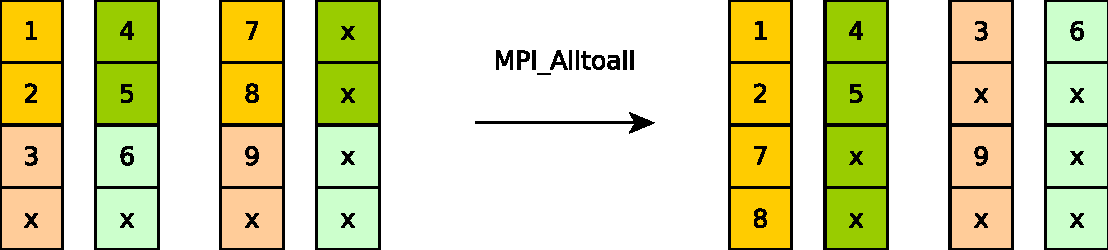
\includegraphics[width=0.8\textwidth]{img/transpose-1.pdf}
  \caption{The result of performing {\tt MPI\_Alltoallv} in the implementation.}
  \label{fig:t1}
\end{figure}

We then perform a local transponation. This works as follows: We perform a local
transponation on each square block we store in memory. The square block's size
has the amount of rows each node contains multiplied with the amount of nodes.
Consequently, each row may be a bit larger than the original $m$, with the
result of a simpler transpose implementation which may be potentially faster
than using {\tt Alltoallv}.

\begin{figure}[h]
  \centering
  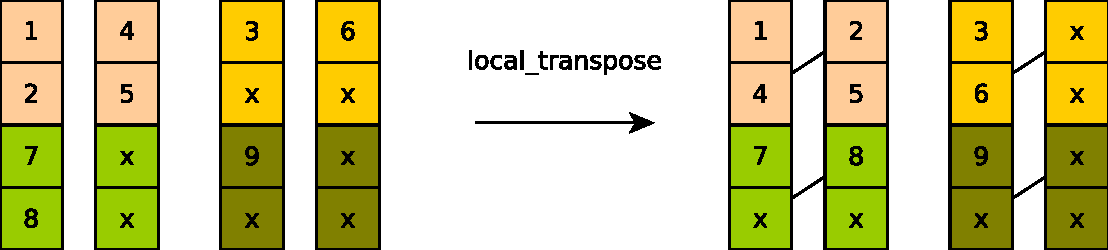
\includegraphics[width=0.8\textwidth]{img/transpose-2.pdf}
  \caption{Performing {\tt local\_transpose} in the implementation.}
  \label{fig:t2}
\end{figure}

In order to load balance as much as possible, the last node will potentially do
less work than the other nodes, compared to the other scenario where it has to
perform more work. Both Figure \ref{fig:t1} and \ref{fig:t2} shows the edge case
where the last node has not as many rows to work with as the previous nodes.

\section{Results}

\begin{table}[H]
   \centering
    \begin{tabular}{| l | l | l | l | l | l |}
    \hline
    \bf{n} & \bf{Nodes} & \bf{Threads} & \bf{Average time} & \bf{Average }$S_{p}$ & \bf{Efficiency} \\ \hline
    	16384 & 1 & 1 & 788.65 & 1 & 1 \\ \hline
	16384 & 3 & 12 & 45.91 & 17.18 & 0.48 \\ \hline
	16384 & 3 & 3 & 33.80 & 23.33 & 0.65 \\ \hline
	16384 & 3 & 1 & 31.11 & 25.35 & 0.70  \\
    \hline
    \end{tabular}
\end{table}
\section{Discussion}

Diskturer: Vi bruker kun ene programmet med openmp og en tråd.

Diskus: alltoall vs alltoallv


\end{document}
